\documentclass{article}

\usepackage{arxiv}

\usepackage[utf8]{inputenc} % allow utf-8 input
\usepackage[T1]{fontenc}    % use 8-bit T1 fonts
\usepackage{hyperref}       % hyperlinks
\usepackage{url}            % simple URL typesetting
\usepackage{booktabs}       % professional-quality tables
\usepackage{amsfonts}       % blackboard math symbols
\usepackage{nicefrac}       % compact symbols for 1/2, etc.
\usepackage{microtype}      % microtypography
\usepackage{lipsum}		% Can be removed after putting your text content
\usepackage{amssymb,amsmath}
\usepackage{listings}
\usepackage{graphicx}
\usepackage{subfig}
\usepackage{apacite}

\title{Contact-tracing strategies for SARS-CoV-2 eradication
\textbf{**** UNFINISHED DRAFT ****}
}

%\date{September 9, 1985}	% Here you can change the date presented in the paper title
%\date{} 					% Or removing it

\author{
  Daniel Tang\\
  Leeds Institute for Data Analytics\thanks{This project has received funding from the European Research Council (ERC) under the European Union’s Horizon 2020 research and innovation programme (grant agreement No. 757455)}\\
  University of Leeds\\
  Leeds, UK\\
  \texttt{D.Tang@leeds.ac.uk} \\
  %% examples of more authors
  %% \AND
  %% Coauthor \\
  %% Affiliation \\
  %% Address \\
}


\begin{document}
\maketitle

\begin{abstract}
As of $27^{th}$ March a large and increasing proportion of the global population are living under social distancing measures in order to control the spread of COVID-19. If these measures are successful we will, in a few months, be in a situation where prevalence is again low in certain parts of the world, however, it is not clear what the best policy will be at that point. This paper investigates the feasibility of using contact tracing along with a combination of other measures in order to ease the social distancing measures while preventing a resurgence of the disease.

\textbf{**** THIS IS UNFINISHED RESEARCH WHICH MAY CONTAIN ERRORS AND IS SUBJECT TO CHANGE ****}
\end{abstract}

% keywords can be removed
\keywords{COVID-19, SARS-CoV-2}

\section{Introduction}

Many countries in the world are now committed to a surge in incidence of COVID-19 and are practising social distancing in order to suppress its spread. If successful, these countries will soon be in a situation where prevalence is reducing. Once this is achieved there are a number of strategies:
\begin{itemize}

\item lift the social distancing measures and allow a second (and subsequent) waves until herd immunity is achieved\cite{ferguson2020impact}.

\item maintain low levels until a vaccine is available

\item eradicate the virus locally and impose strict border controls and containment strategies until the virus is contained globally
\end{itemize}

Here we investigate the feasibility of the third option by slowly lifting social distancing measures while maintaining self isolation of symptomatic individuals and implementing an extensive testing and contact-tracing capability.

\section{Description of the Model}

The model we use is an agent-based discrete event simulation. It is based on the stochastic branching model described in \cite{hellewellfeasibility} but modified in order to capture enough detail to explore different testing and contact-tracing strategies while capturing the workload on a centralised testing and contact-tracing facility and the increasing delays in this facility as workload increases.\footnote{Although a discrete-event simulation is slower than a branching model, execution time is not a bottleneck so it is worthwhile in order to capture the dynamics.}

The model consists of infected agents, each of which belongs to a household and a workplace/school. Once infected, an agent goes though an incubation period with duration drawn from a Weibull distribution (with shape parameter $2.322737$ and scale parameter $6.492272$)\cite{backer2020incubation}. The transmission serial interval (i.e. time from exposure to transmission) is drawn from a skew normal distribution with location parameter equal to the clinical onset time (i.e. end of the incubation period), scale parameter of 2.0 and skew parameter of 1.95\cite{hellewellfeasibility}. This results in 15\% of infections occurring before clinical onset\cite{hellewellfeasibility}. In order to avoid unrealistically early transmissions, the serial interval was bounded to a minimum of 1 day. At creation, $17.9\%$ of agents are deemed to be asymptomatic\cite{:/content/10.2807/1560-7917.ES.2020.25.10.2000180}\footnote{[TODO: Age weight this figure]}. Asymptomatic carriers are assumed to be $\frac{2}{3}$ as infectious as symptomatic carriers\cite{ferguson2020impact}. The number of susceptible agents that an infected agent will infect if not isolated is drawn from a negative binomial distribution with overdispersion parameter $10.0$\cite{zhuang2020preliminary}\cite{riou2020pattern} and mean of $\frac{3R_0}{3 - \rho}$ for symptomatic agents and $\frac{2R_0}{3 - \rho}$ for asymptomatic agents where $\rho=0.179$ is the probability of being asymptomatic and $R_0$ is the basic reproductive number. At each transmission event a new infected agent is created, unless the agent is isolated, in which case the event has no effect.

Each transmission event occurs either in the household, at the workplace/school or in the community. This allows us to capture the differences in ease and speed of contact tracing in these three cases, and to capture the effect of different policies for tracing in these contexts. It also allows us to capture the effect of household-wide self-isolation policies such as those implemented in the UK. The relative probability of transmission in the three locations was calibrated in order to obtain equal aggregate numbers of transmission events in each location\cite{ferguson2020impact}. The distribution of number of members in a household was calibrated against\cite{smithHouseholds}.

In order to account for people who have already been infected during the first wave of infection, a proportion of the population is immune to infection. A transmission event to an immune agent does not cause infection. This immunity is applied only to school/workplace and community under the assumption that, during the peak, under ``stay at home'' rules during the initial peak of infections, if one member of a household contracts the disease it is highly likely that all other members will also contract it, and so the whole household will become immune. This means that only members of non-immune households can subsequently become infected.

\subsection{Contact tracing and isolation policy}

It was assumed that a ``self-isolate'' policy was in place such that anyone who becomes symptomatic must self-isolate and report to authorities. At this point all members of that person's household must also self-isolate. It was assumed that there was a delay between symptom onset and self-isolation/reporting. Once reported, all members of the household are tested and those that test positive are contact-traced. Contact tracing was assumed to identify $90\%$ of contacts in the workplace/school and $10\%$ of contacts in the community. Symptomatic contacts in the workplace must isolate immediately, other contacts are tested and must isolate on positive test result. The time from being tested to getting a result was assumed to be 24 hours. Tests were positive if the infectiveness of the agent at the time of the test was above $2\%$ per day, this encompassed the vast majority of the infective period, but excluded the latent period. It was assumed that $10\%$ of the population do not comply with these rules and never self-isolate or report themselves.

The source code of the model is available at \href{https://github.com/danftang/Covid19}{https://github.com/danftang/Covid19}

\section{Policy Scenarios}

Various policy scenarios were simulated to find the probability that an initial population of 100 infected agents could be eradicated. Eradication was deemed to have been achieved if the cumulative number of cases remained below 5000 and there was no untraced infected population at 15 weeks into the simulation. It was assumed that $5\%$ of the population was immune. The probability of eradication was estimated by performing a monte-carlo run of 300 simulations and counting the proportion that achieved eradication.

\subsection{No contact tracing, self isolation}

Ordering people to self-isolate upon becoming symptomatic is unlikely to work on its own. The only chance of containment is if isolation occurs immediately on symptom onset. Figure \ref{noTracing} shows the case when 15\% of transmission is pre-symptomatic and there is 90\% compliance. This kind of compliance so quickly after symptom onset would only be practical under legal enforcement and close monitoring (e.g. thermal cameras, social stigma, fines etc.) and would only work if R0 is on the low side of the feasible range.

\begin{figure}
\begin{center}
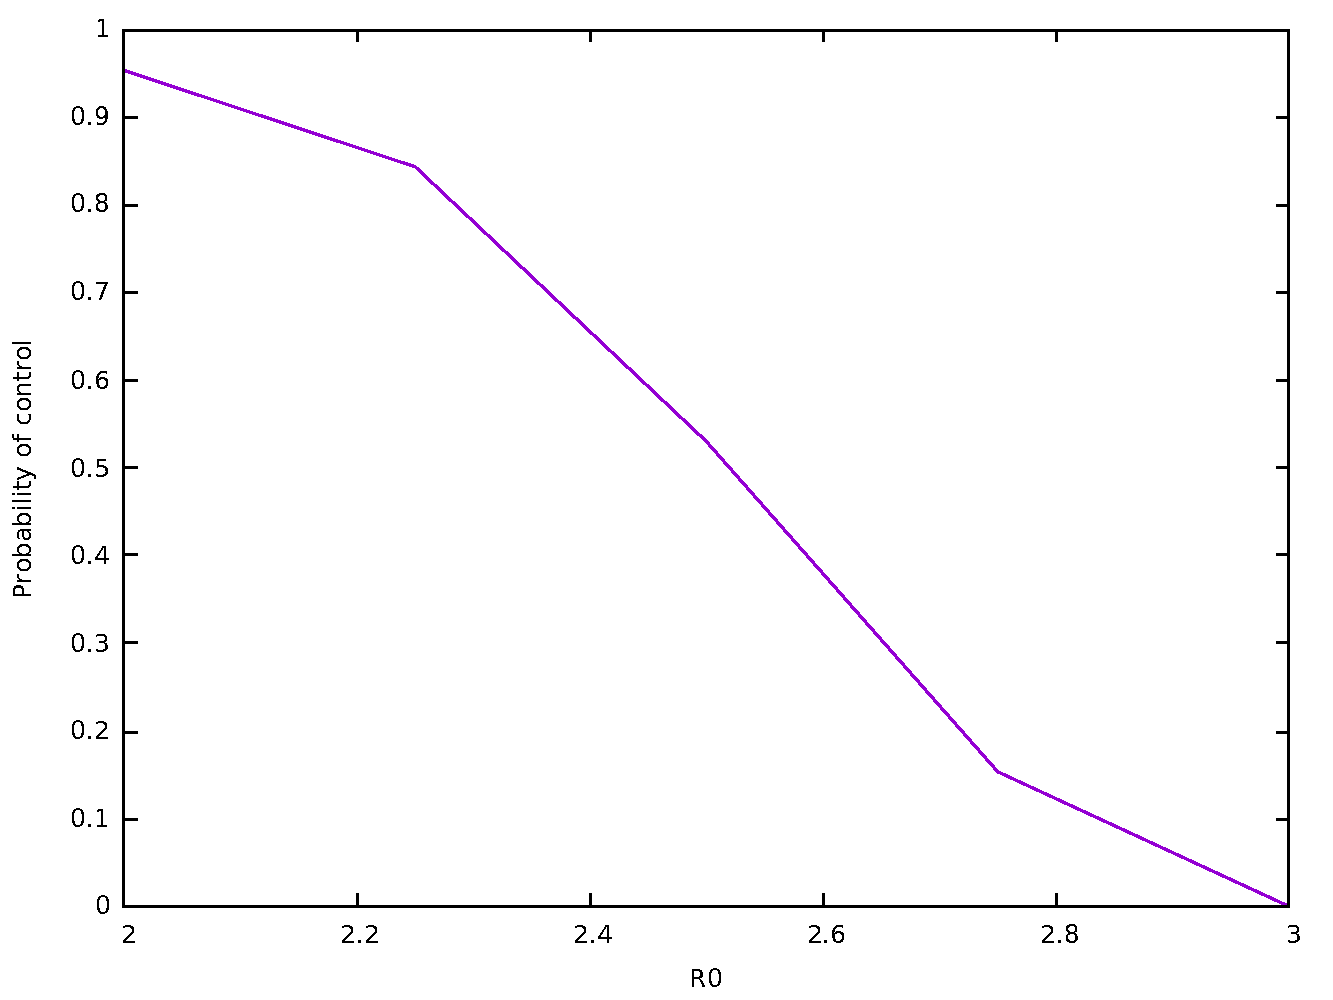
\includegraphics[width = 10cm]{noTracingR0.pdf}
\end{center}
\caption{Probability of eradication under self-isolation only assuming 90\% compliance and 15\% pre-symptomatic transmission.}
\label{noTracing}
\end{figure}

\subsection{Whole household isolation}

Ordering a whole household to self-isolate upon any member becoming symptomatic is more effective (Figure \ref{householdQuarantine}) but still not probable enough to be a good strategy.

\begin{figure}
\begin{center}
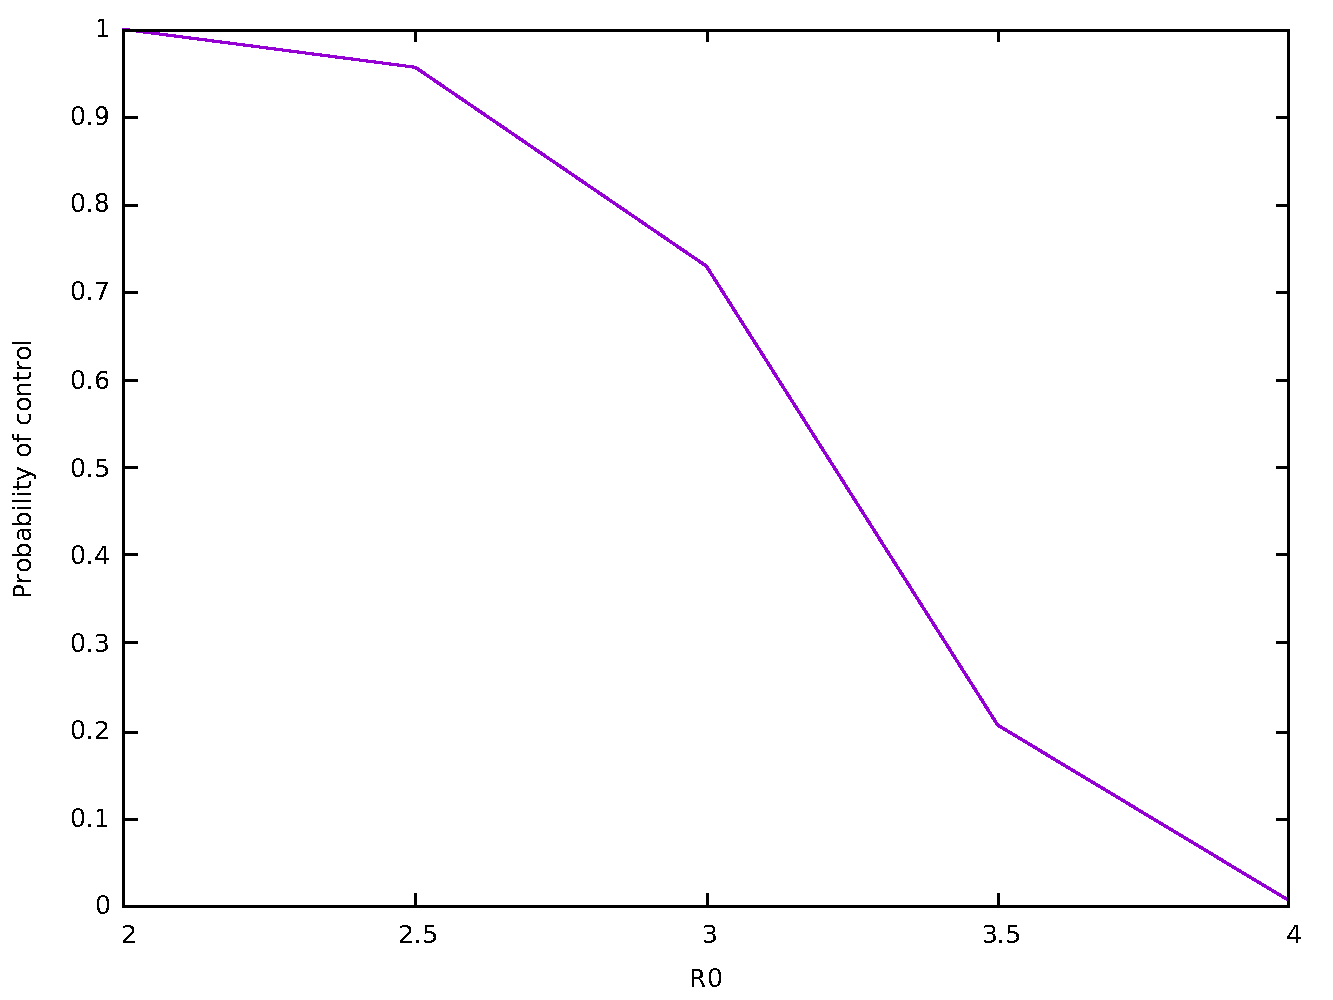
\includegraphics[width = 10cm]{householdQuarantineR0.pdf}
\end{center}
\caption{Probability of eradication under whole household quarantine assuming 90\% compliance and 15\% pre-symptomatic transmission.}
\label{householdQuarantine}
\end{figure}

\subsection{Isolation of whole household and work-colleagues}

Ordering both the household and close contacts at work to be isolated could work under some parameter values. In this scenario, close contacts of a symptomatic at home and work would immediately be asked to self-isolate and take a swab test. Those that tested positive (after a 24 hour delay) would themselves require their whole household and work contacts to also isolate and take a swab test and so on. By instating a legal requirement for companies to force traced contacts to stay (and if possible work) from home and by making it a duty for companies to report symptomatic employees it is feasible that the time from onset to isolation can be made small while making compliance high. Figure \ref{householdWorkplace15} shows that with $R0 \le 3$ and $15\%$ pre-symptomatic transmission then this strategy would have a high chance of success given 90\% compliance. However, at a pre-symptomatic transmission of $50\%$ this strategy looks less feasible (figure \ref{householdWorkplace50}).

\begin{figure}
\begin{center}
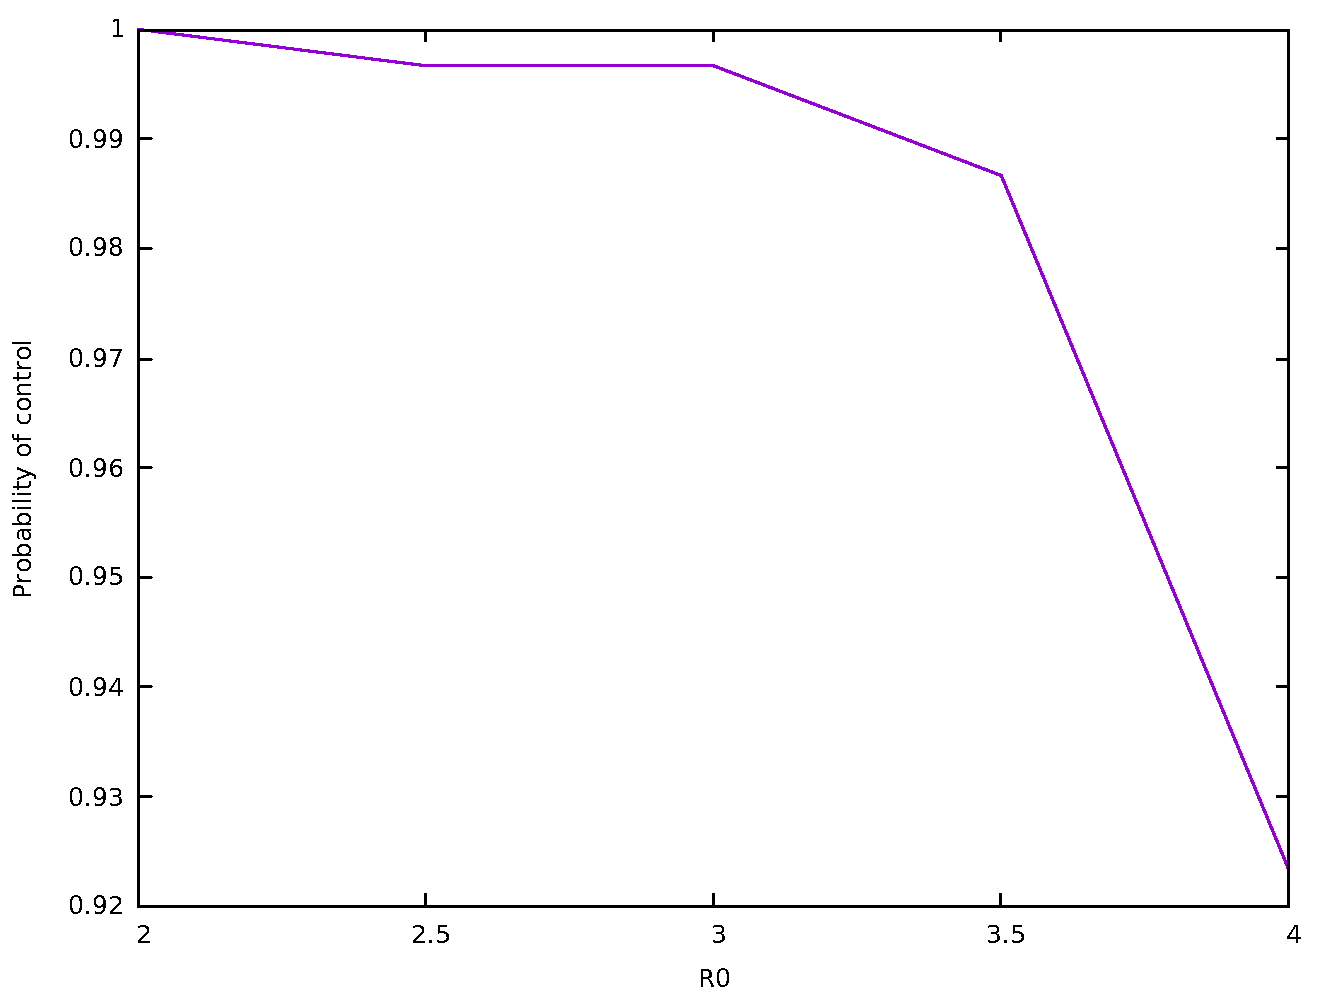
\includegraphics[width = 10cm]{householdAndWorkplace15pre.pdf}
\end{center}
\caption{Probability of eradication under quarantine of whole household and workplace contacts assuming 90\% compliance and 15\% pre-symptomatic transmission.}
\label{householdWorkplace15}
\end{figure}

\begin{figure}
\begin{center}
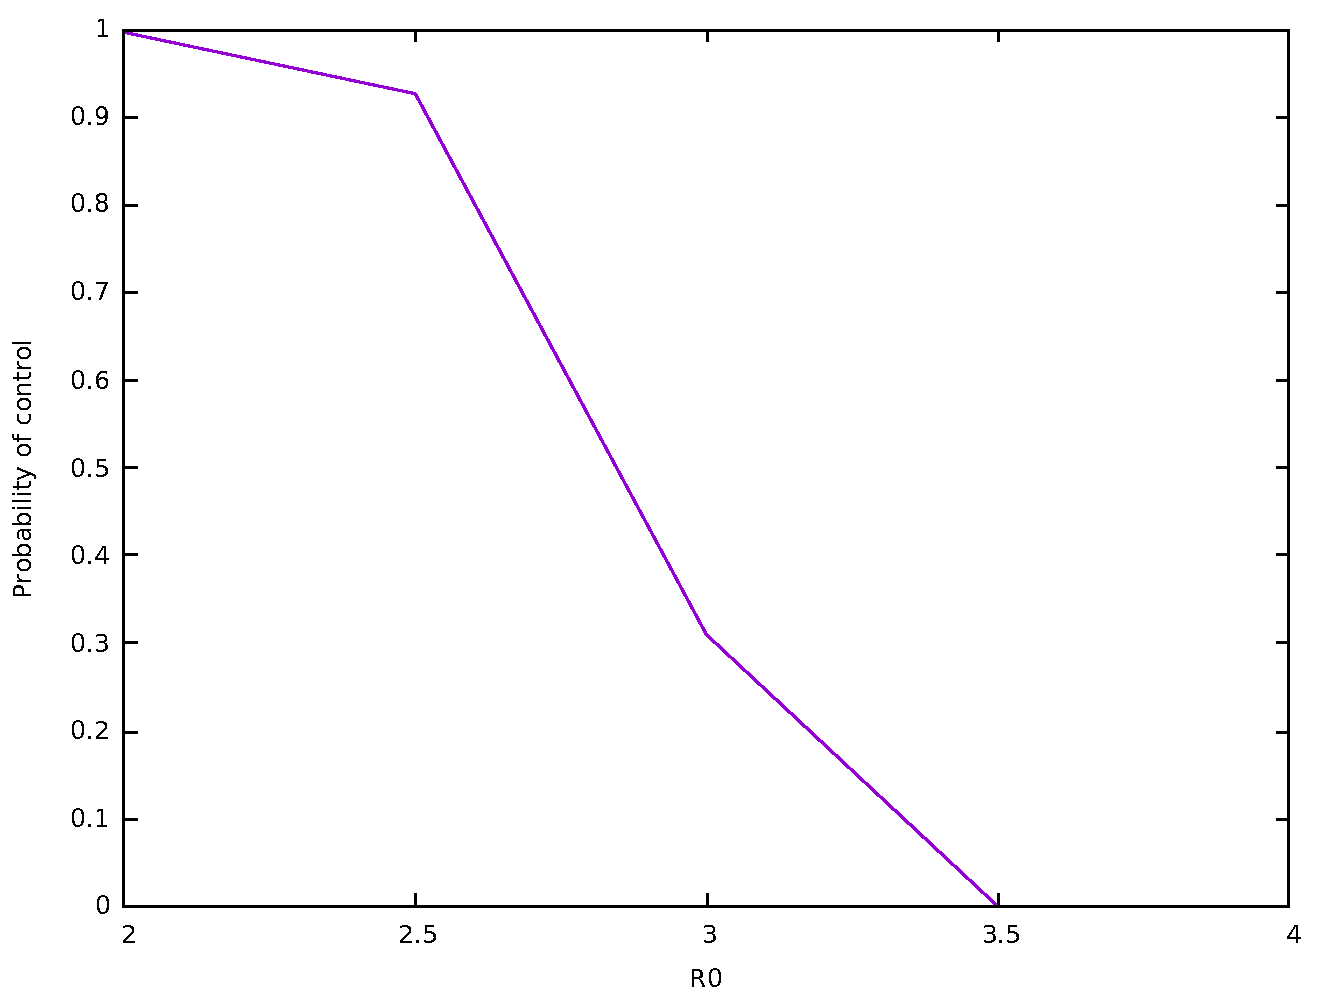
\includegraphics[width = 10cm]{householdAndWorkplace50pre.pdf}
\end{center}
\caption{Probability of eradication under quarantine of whole household and workplace contacts assuming 90\% compliance and 50\% pre-symptomatic transmission.}
\label{householdWorkplace50}
\end{figure}

\subsection{Community contact tracing}

If, in addition to household and workplace tracing, contacts could also be traced in the community, and told to isolate and take a swab test if they had been in close contact with a person who later tested positive, then there is a good chance of success even in the case of $R0 = 3.5$ and $50\%$ pre-symptomatic transmission, see figures \ref{fulltrace2.5} and \ref{fulltrace3.5}.

However, even under this scenario, we need 80\% compliance in the community, in addition to enforcement at work, to have a good chance of success.

\begin{figure}
\begin{center}
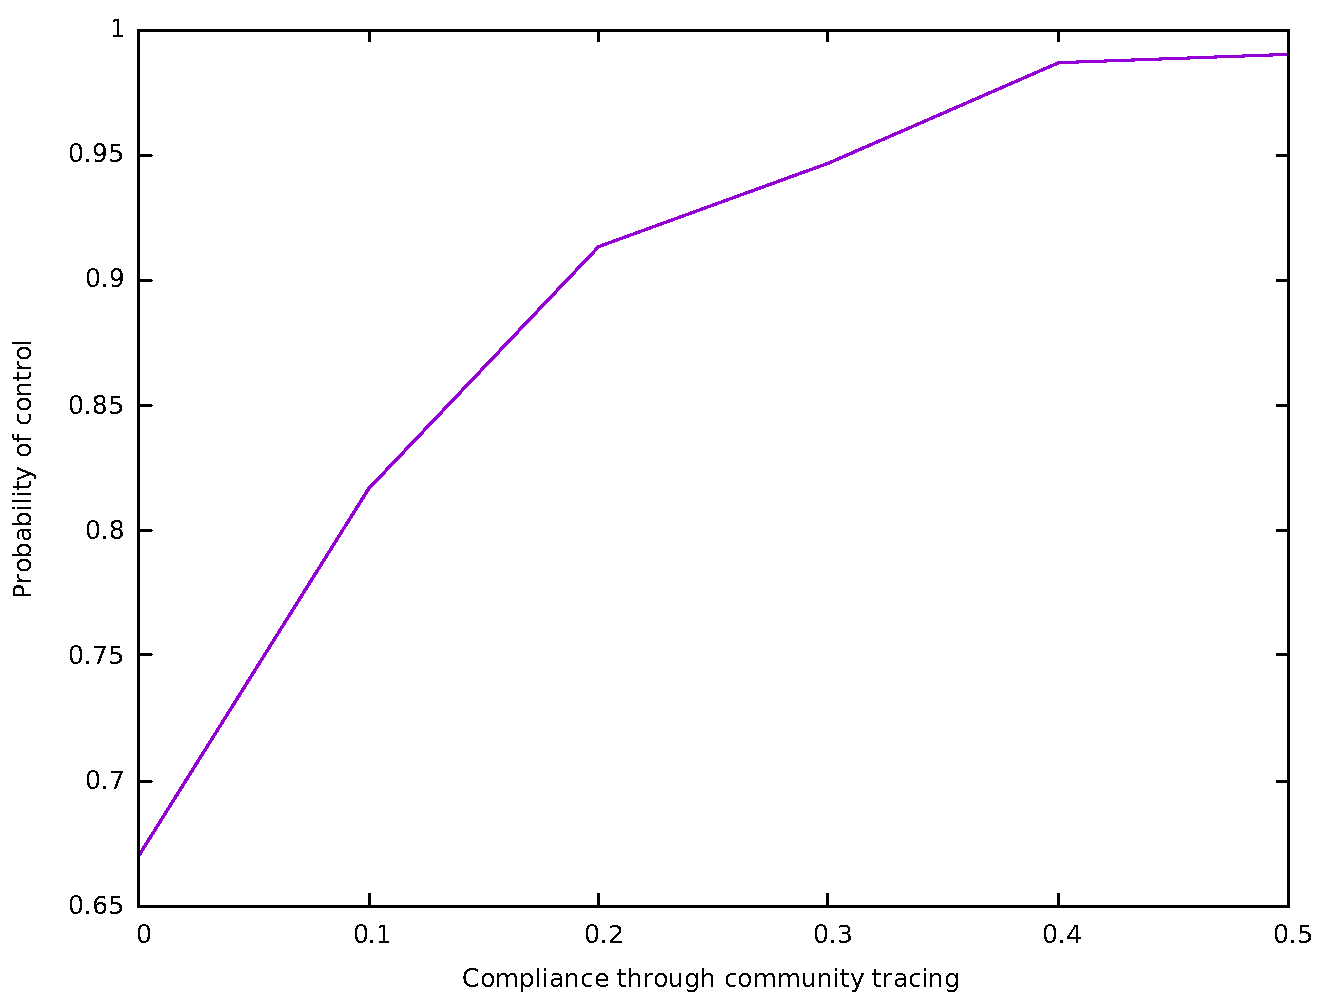
\includegraphics[width = 10cm]{fullTrace50pre25R0.pdf}
\end{center}
\caption{Probability of eradication under community tracing assuming 90\% self-report compliance, 50\% pre-symptomatic transmission and $R0 = 2.5$.}
\label{fulltrace2.5}
\end{figure}

\begin{figure}
\begin{center}
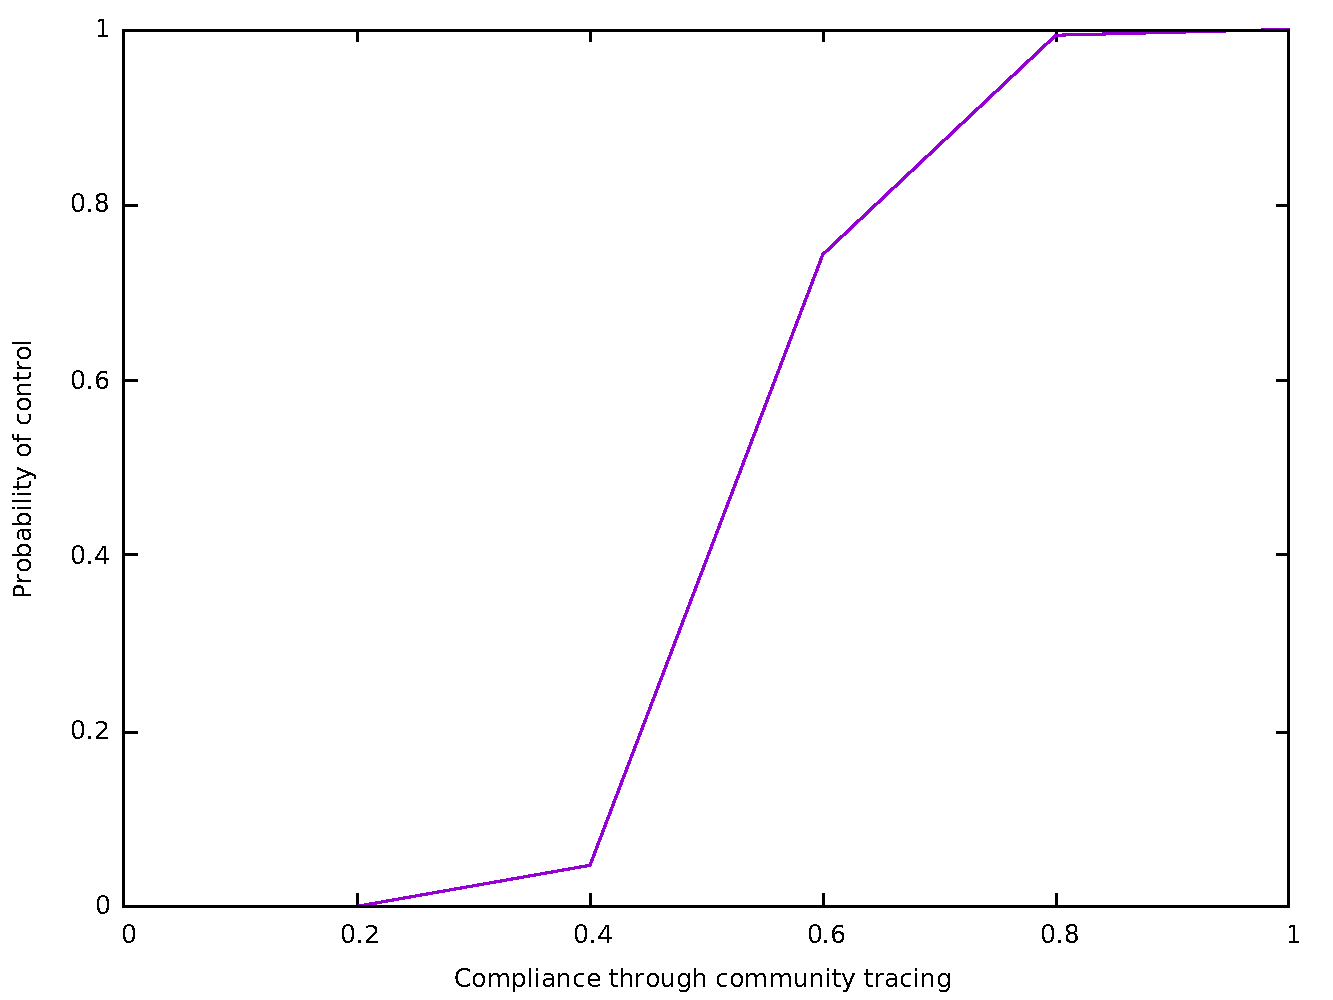
\includegraphics[width = 10cm]{fullTrace50pre35R0.pdf}
\end{center}
\caption{Probability of eradication under community tracing assuming 90\% self-report compliance, 50\% pre-symptomatic transmission and $R0 = 3.5$.}
\label{fulltrace3.5}
\end{figure}

\section{Contact tracing in the community while maintaining privacy}

Achieving contact tracing that is fast and efficient enough to make the above strategy feasible will require a technological solution, probably by leveraging mobile phones. For any such contact-tracing strategy to be acceptable in the context of a western democracy, the privacy of the participants is of paramount importance. For that reason we suggest the following technological solution to contact tracing:

Each participant must have a mobile phone equipped with Bluetooth and an Internet connection. An app will be installed which turns on the phone's Bluetooth connection. To maintain anonymity, the Bluetooth MAC address will be spoofed to a randomly chosen 48-bit number\footnote{Is this possible?}. The chosen number will be locally stored in the app. If another phone with the app installed comes close for more than a fixed amount of time, then the two will be classed as a ``close contact'' and each phone will store the MAC address of the other's along with it's own MAC address. At intervals of, say, 2 minutes, the MAC address will be changed to a new, randomly chosen number.

As a person travels through the community, the app will collect the temporary MAC addresses of all close contacts, along with the MAC addresses that it spoofed. Because these are randomly generated numbers there is no way to identify anyone or track their movements from the temporary MAC addresses.

If a person tests positive, all the MAC addresses on that person's phone will be made public on the Internet. Since these are just random numbers, no sensitive information is disclosed. Periodically, all apps will check the published numbers against it's own locally stored record of the MAC addresses that it has spoofed. If there is a match, the user can be notified that they are at risk and should self-isolate and be tested.

In this way, all close contacts of a newly confirmed case (as long as they are using the app) can immediately be informed that they are at risk. The only limitation being the uptake of the app and the compliance of the user with advice to self isolate.

In order to encourage people to install the app public shops and buildings could require the app to be installed in order to gain entry[?].

\section{Discussion}

These early results are subject to further calibration of the model and are likely to change as our understanding of the dynamics of SARS-CoV-2 develops. It also remains to do a proper sensitivity analysis of the model (particularly sensitivity to the proportion of asymptomatics), and to properly treat uncertainty, which is large.

However, the results indicate that contact tracing in the community will be necessary to have a good chance of eradication. We have presented a technological solution to achieve the speed and accuracy needed to make this possible, while maintaining the privacy of users.

%\bibliographystyle{unsrtnat}
%\bibliographystyle{apalike} 
\bibliographystyle{apacite}
\bibliography{references}

\end{document}
